\documentclass{standalone}
\usepackage{tikz}
\usetikzlibrary{patterns, positioning}
\usepackage[sfdefault]{ClearSans} %% option 'sfdefault' activates Clear Sans as the default text font
\usepackage[T1]{fontenc}

\begin{document}
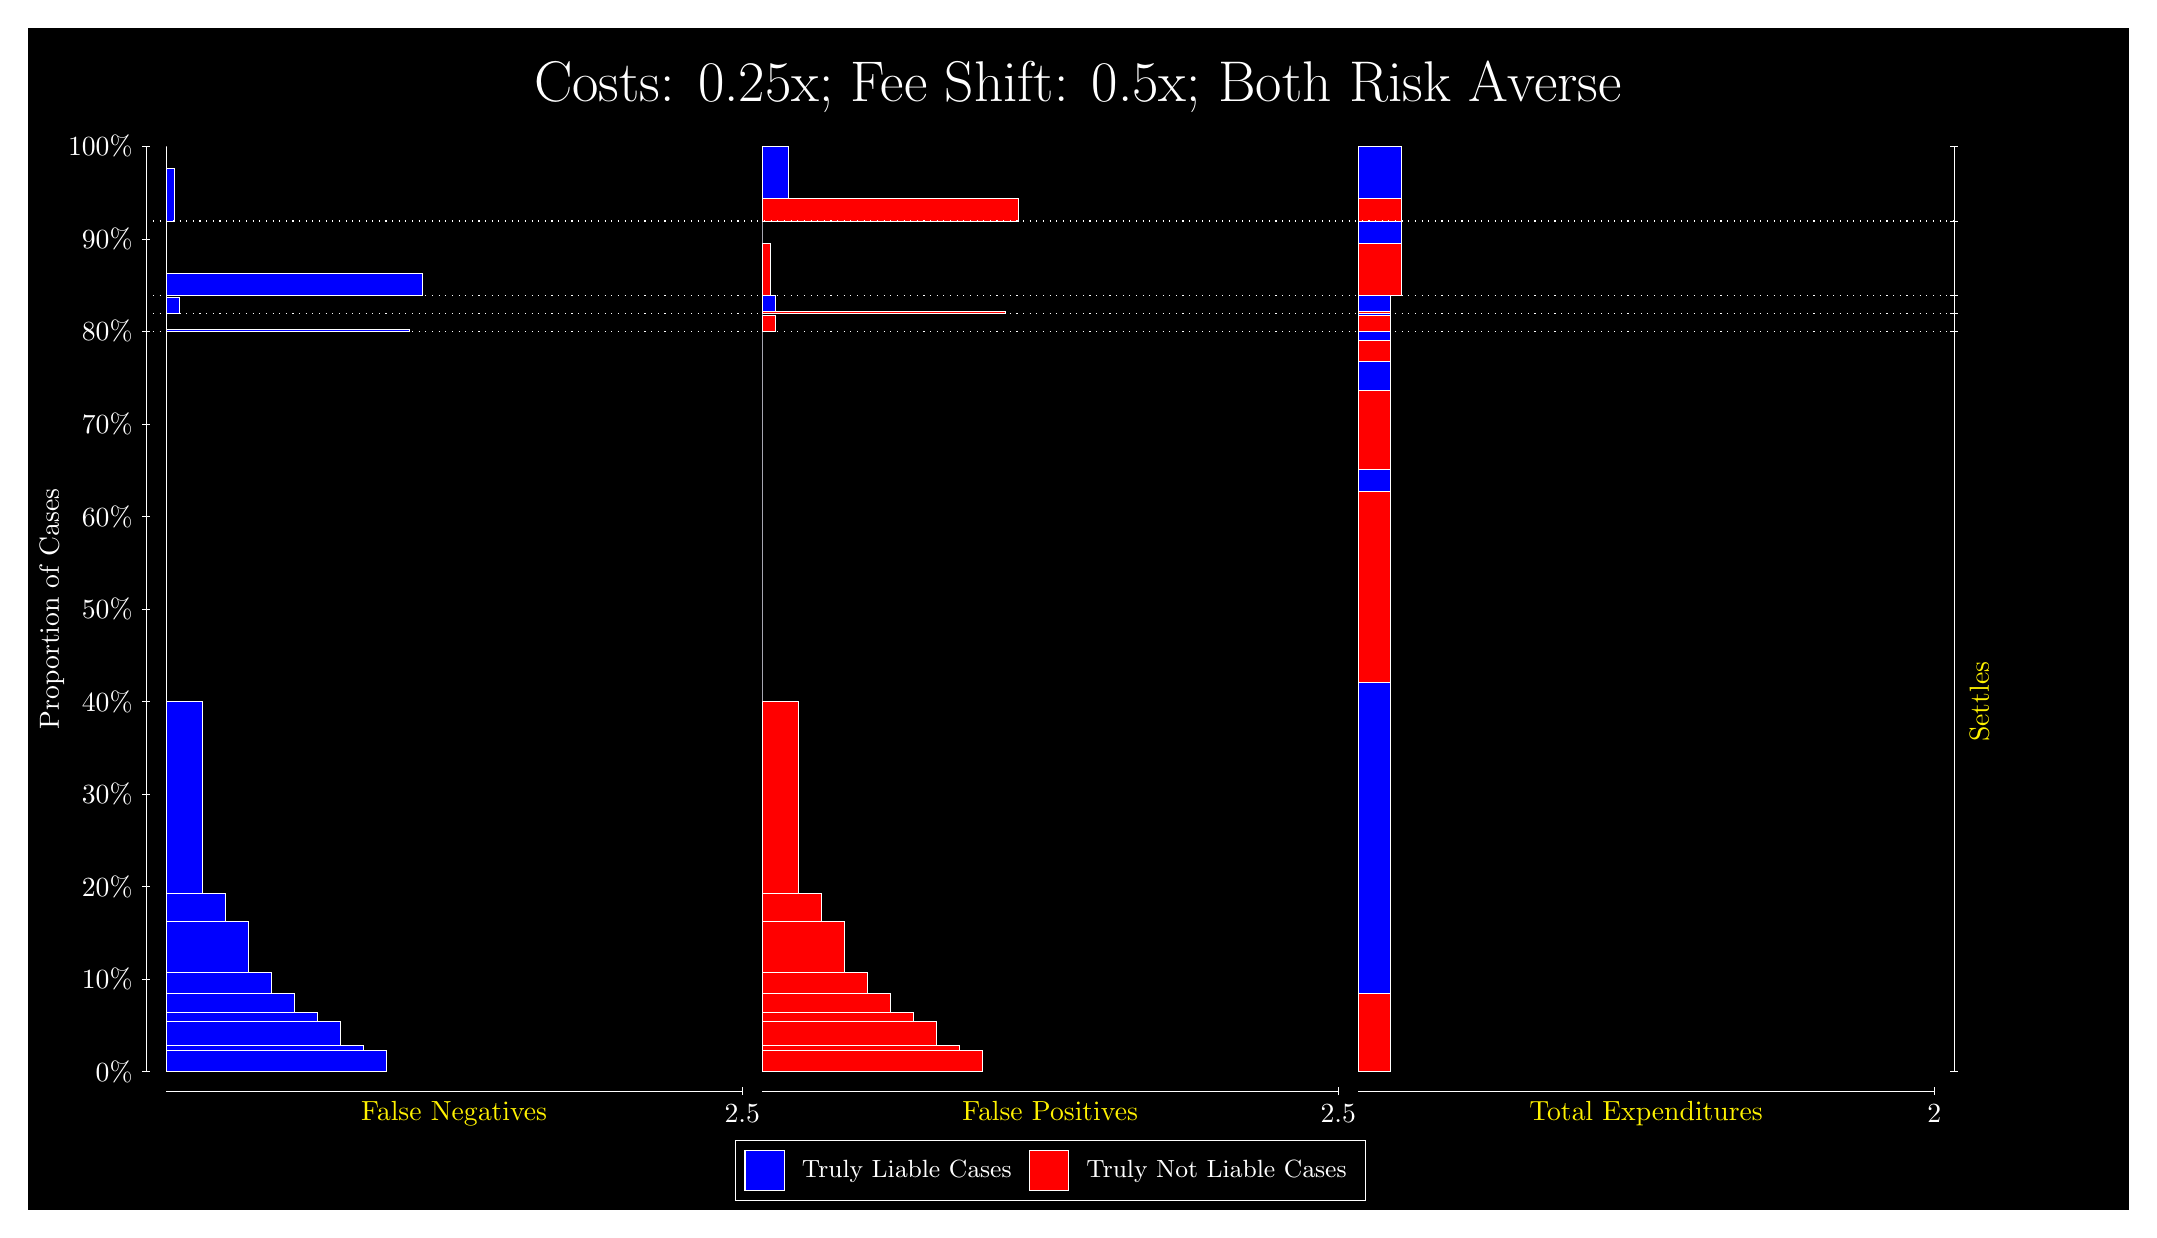
\begin{tikzpicture}
\draw[fill=black] (0,0) rectangle (26.667,15);
\draw[text=white] (0,13.5) rectangle (26.667,15) node[midway] {\huge Costs: 0.25x; Fee Shift: 0.5x; Both Risk Averse};
\draw[white, very thin] (1.5,1.75) -- (1.5,13.5);
\node[rotate=90, text=white, anchor=center] at (0.3, 7.625) {Proportion of Cases};
\draw[white, very thin] (1.45,1.75) -- (1.55,1.75);
\node[text=white, anchor=east] at (1.45, 1.75) {0\%};
\draw[white, very thin] (1.45,2.925) -- (1.55,2.925);
\node[text=white, anchor=east] at (1.45, 2.925) {10\%};
\draw[white, very thin] (1.45,4.1) -- (1.55,4.1);
\node[text=white, anchor=east] at (1.45, 4.1) {20\%};
\draw[white, very thin] (1.45,5.275) -- (1.55,5.275);
\node[text=white, anchor=east] at (1.45, 5.275) {30\%};
\draw[white, very thin] (1.45,6.45) -- (1.55,6.45);
\node[text=white, anchor=east] at (1.45, 6.45) {40\%};
\draw[white, very thin] (1.45,7.625) -- (1.55,7.625);
\node[text=white, anchor=east] at (1.45, 7.625) {50\%};
\draw[white, very thin] (1.45,8.8) -- (1.55,8.8);
\node[text=white, anchor=east] at (1.45, 8.8) {60\%};
\draw[white, very thin] (1.45,9.975) -- (1.55,9.975);
\node[text=white, anchor=east] at (1.45, 9.975) {70\%};
\draw[white, very thin] (1.45,11.15) -- (1.55,11.15);
\node[text=white, anchor=east] at (1.45, 11.15) {80\%};
\draw[white, very thin] (1.45,12.325) -- (1.55,12.325);
\node[text=white, anchor=east] at (1.45, 12.325) {90\%};
\draw[white, very thin] (1.45,13.5) -- (1.55,13.5);
\node[text=white, anchor=east] at (1.45, 13.5) {100\%};

\draw[white, very thin] (24.457,1.75) -- (24.457,13.5);
\draw[white, very thin] (24.407,1.75) -- (24.507,1.75);
\node[anchor=west] at (24.407, 1.75) {};
\draw[white, very thin] (24.407,11.145) -- (24.507,11.145);
\node[anchor=west] at (24.407, 11.145) {};
\draw[white, very thin] (24.407,11.375) -- (24.507,11.375);
\node[anchor=west] at (24.407, 11.375) {};
\draw[white, very thin] (24.407,11.604) -- (24.507,11.604);
\node[anchor=west] at (24.407, 11.604) {};
\draw[white, very thin] (24.407,12.552) -- (24.507,12.552);
\node[anchor=west] at (24.407, 12.552) {};
\draw[white, very thin] (24.407,13.5) -- (24.507,13.5);
\node[anchor=west] at (24.407, 13.5) {};

\draw[white, very thin, fill=blue] (1.75,1.75) rectangle (4.5495,2.0236);
\draw[white, very thin, fill=blue] (1.75,2.0236) rectangle (4.2567,2.0889);
\draw[white, very thin, fill=blue] (1.75,2.0889) rectangle (3.964,2.3864);
\draw[white, very thin, fill=blue] (1.75,2.3864) rectangle (3.6712,2.4995);
\draw[white, very thin, fill=blue] (1.75,2.4995) rectangle (3.3784,2.7434);
\draw[white, very thin, fill=blue] (1.75,2.7434) rectangle (3.0857,3.0046);
\draw[white, very thin, fill=blue] (1.75,3.0046) rectangle (2.7929,3.6546);
\draw[white, very thin, fill=blue] (1.75,3.6546) rectangle (2.5002,4.0193);
\draw[white, very thin, fill=blue] (1.75,4.0193) rectangle (2.2074,6.4476);
\draw[white, very thin, fill=red] (1.75,6.4476) rectangle (1.75,11.145);
\draw[white, very thin, fill=blue] (1.75,11.145) rectangle (4.8422,11.171);
\draw[white, very thin, fill=red] (1.75,11.171) rectangle (1.75,11.375);
\draw[white, very thin, fill=blue] (1.75,11.375) rectangle (1.9147,11.578);
\draw[white, very thin, fill=red] (1.75,11.578) rectangle (1.75,11.604);
\draw[white, very thin, fill=blue] (1.75,11.604) rectangle (5.0069,11.886);
\draw[white, very thin, fill=red] (1.75,11.886) rectangle (1.75,12.552);
\draw[white, very thin, fill=blue] (1.75,12.552) rectangle (1.8598,13.218);
\draw[white, very thin, fill=red] (1.75,13.218) rectangle (1.75,13.5);
\draw[white, very thin, fill=red] (9.3189,1.75) rectangle (12.118,2.0236);
\draw[white, very thin, fill=red] (9.3189,2.0236) rectangle (11.826,2.0889);
\draw[white, very thin, fill=red] (9.3189,2.0889) rectangle (11.533,2.3864);
\draw[white, very thin, fill=red] (9.3189,2.3864) rectangle (11.24,2.4995);
\draw[white, very thin, fill=red] (9.3189,2.4995) rectangle (10.947,2.7434);
\draw[white, very thin, fill=red] (9.3189,2.7434) rectangle (10.655,3.0046);
\draw[white, very thin, fill=red] (9.3189,3.0046) rectangle (10.362,3.6546);
\draw[white, very thin, fill=red] (9.3189,3.6546) rectangle (10.069,4.0193);
\draw[white, very thin, fill=red] (9.3189,4.0193) rectangle (9.7763,6.4477);
\draw[white, very thin, fill=blue] (9.3189,6.4477) rectangle (9.3189,11.145);
\draw[white, very thin, fill=red] (9.3189,11.145) rectangle (9.4835,11.349);
\draw[white, very thin, fill=blue] (9.3189,11.349) rectangle (9.3189,11.375);
\draw[white, very thin, fill=red] (9.3189,11.375) rectangle (12.411,11.4);
\draw[white, very thin, fill=blue] (9.3189,11.4) rectangle (9.4835,11.604);
\draw[white, very thin, fill=red] (9.3189,11.604) rectangle (9.4287,12.269);
\draw[white, very thin, fill=blue] (9.3189,12.269) rectangle (9.3189,12.552);
\draw[white, very thin, fill=red] (9.3189,12.552) rectangle (12.576,12.834);
\draw[white, very thin, fill=blue] (9.3189,12.834) rectangle (9.6482,13.5);
\draw[white, very thin, fill=red] (16.888,1.75) rectangle (17.299,2.7434);
\draw[white, very thin, fill=blue] (16.888,2.7434) rectangle (17.299,6.6915);
\draw[white, very thin, fill=red] (16.888,6.6915) rectangle (17.299,9.1199);
\draw[white, very thin, fill=blue] (16.888,9.1199) rectangle (17.299,9.3934);
\draw[white, very thin, fill=red] (16.888,9.3934) rectangle (17.299,10.408);
\draw[white, very thin, fill=blue] (16.888,10.408) rectangle (17.299,10.771);
\draw[white, very thin, fill=red] (16.888,10.771) rectangle (17.299,11.032);
\draw[white, very thin, fill=blue] (16.888,11.032) rectangle (17.299,11.145);
\draw[white, very thin, fill=red] (16.888,11.145) rectangle (17.299,11.349);
\draw[white, very thin, fill=blue] (16.888,11.349) rectangle (17.299,11.375);
\draw[white, very thin, fill=red] (16.888,11.375) rectangle (17.299,11.4);
\draw[white, very thin, fill=blue] (16.888,11.4) rectangle (17.299,11.604);
\draw[white, very thin, fill=red] (16.888,11.604) rectangle (17.437,12.269);
\draw[white, very thin, fill=blue] (16.888,12.269) rectangle (17.437,12.552);
\draw[white, very thin, fill=red] (16.888,12.552) rectangle (17.437,12.834);
\draw[white, very thin, fill=blue] (16.888,12.834) rectangle (17.437,13.5);
\draw[white, dotted] (1.5,11.145) -- (24.457,11.145);
\draw[white, dotted] (1.5,11.375) -- (24.457,11.375);
\draw[white, dotted] (1.5,11.604) -- (24.457,11.604);
\draw[white, dotted] (1.5,12.552) -- (24.457,12.552);
\draw[white, very thin] (1.75,1.5) -- (9.0689,1.5);
\node[text=yellow, anchor=north] at (5.4094, 1.5) {False Negatives};
\draw[white, very thin] (9.0689,1.45) -- (9.0689,1.55);
\node[text=white, anchor=north] at (9.0689, 1.45) {2.5};

\draw[white, very thin] (9.3189,1.5) -- (16.638,1.5);
\node[text=yellow, anchor=north] at (12.978, 1.5) {False Positives};
\draw[white, very thin] (16.638,1.45) -- (16.638,1.55);
\node[text=white, anchor=north] at (16.638, 1.45) {2.5};

\draw[white, very thin] (16.888,1.5) -- (24.207,1.5);
\node[text=yellow, anchor=north] at (20.547, 1.5) {Total Expenditures};
\draw[white, very thin] (24.207,1.45) -- (24.207,1.55);
\node[text=white, anchor=north] at (24.207, 1.45) {2};

\node[text=yellow, centered, rotate=90] at (24.777, 6.4477) {Settles};





\draw (12.978300999999998,1.5) node[draw=none] (baseCoordinate) {};
\begin{scope}[align=center]
        \matrix[scale=0.5, draw=white, below=0.5cm of baseCoordinate, nodes={draw}, column sep=0.1cm]{
            \node[rectangle, draw, minimum width=0.5cm, minimum height=0.5cm, fill=blue] {}; &
            \node[draw=none, font=\small, text=white] (B) {Truly Liable Cases}; &
            \node[rectangle, draw, minimum width=0.5cm, minimum height=0.5cm, fill=red] {}; &
            \node[draw=none, font=\small, text=white] (B) {Truly Not Liable Cases}; \\
            };
\end{scope}

\end{tikzpicture}
\end{document}